% =============================================================================
% Lecture 05: Multivariate Methods
% BSAD 8310: Business Forecasting
% University of Nebraska at Omaha
% =============================================================================

\documentclass[aspectratio=169, 11pt]{beamer}

% =============================================================================
% header.tex — BSAD 8310: Business Forecasting
% University of Nebraska at Omaha
% Beamer theme: UNO-branded, clean, professional
% =============================================================================

% ----------------------------- BEAMER THEME ----------------------------------
\usetheme{default}
\useinnertheme{rectangles}

% ----------------------------- UNO COLOR PALETTE -----------------------------
\definecolor{unoblue}{HTML}{005CA9}
\definecolor{unored}{HTML}{E41C38}
\definecolor{unogray}{HTML}{525252}
\definecolor{unogreen}{HTML}{15803d}
\definecolor{unolightblue}{HTML}{E8F0FA}
\definecolor{unolightred}{HTML}{FDECEA}
\definecolor{unolightgreen}{HTML}{F0FAF4}
\definecolor{unowhite}{HTML}{FFFFFF}

% Apply UNO colors to Beamer structure
\setbeamercolor{structure}{fg=unoblue}
\setbeamercolor{palette primary}{bg=unoblue, fg=white}
\setbeamercolor{palette secondary}{bg=unoblue!80!black, fg=white}
\setbeamercolor{palette tertiary}{bg=unoblue!60!black, fg=white}
\setbeamercolor{frametitle}{bg=unoblue, fg=white}
\setbeamercolor{frametitle right}{bg=unoblue!80!black}
\setbeamercolor{title}{fg=unoblue}
\setbeamercolor{subtitle}{fg=unogray}
\setbeamercolor{author in head/foot}{bg=unoblue, fg=white}
\setbeamercolor{title in head/foot}{bg=unoblue!80, fg=white}
\setbeamercolor{date in head/foot}{bg=unoblue!60, fg=white}
\setbeamercolor{page number in head/foot}{bg=unoblue!60, fg=white}
\setbeamercolor{block title}{bg=unoblue, fg=white}
\setbeamercolor{block body}{bg=unolightblue}
\setbeamercolor{block title alerted}{bg=unored, fg=white}
\setbeamercolor{block body alerted}{bg=unolightred}
\setbeamercolor{block title example}{bg=unogreen, fg=white}
\setbeamercolor{block body example}{bg=unolightgreen}
\setbeamercolor{itemize item}{fg=unoblue}
\setbeamercolor{itemize subitem}{fg=unored}
\setbeamercolor{enumerate item}{fg=unoblue}
\setbeamercolor{enumerate subitem}{fg=unored}
\setbeamercolor{alerted text}{fg=unored}

% ----------------------------- FONTS -----------------------------------------
\usefonttheme{professionalfonts}
\usefonttheme[onlymath]{serif}       % serif math; sans-serif text
\setbeamerfont{frametitle}{size=\large, series=\bfseries}
\setbeamerfont{title}{size=\LARGE, series=\bfseries}
\setbeamerfont{subtitle}{size=\large}
\setbeamerfont{block title}{size=\normalsize, series=\bfseries}
\setbeamerfont{footline}{size=\tiny}

% ----------------------------- LAYOUT ----------------------------------------
\setbeamersize{text margin left=0.5cm, text margin right=0.5cm}
\setbeamertemplate{navigation symbols}{}   % remove navigation buttons
\setbeamertemplate{itemize items}[circle]
\setbeamertemplate{enumerate items}[default]

% Custom footline: [Course] [Title] [Page/Total]
\setbeamertemplate{footline}{%
  \leavevmode%
  \hbox{%
    \begin{beamercolorbox}[wd=.33\paperwidth, ht=2.5ex, dp=1ex, left, leftskip=4pt]
      {author in head/foot}%
      \usebeamerfont{author in head/foot}\insertshortauthor
    \end{beamercolorbox}%
    \begin{beamercolorbox}[wd=.34\paperwidth, ht=2.5ex, dp=1ex, center]
      {title in head/foot}%
      \usebeamerfont{title in head/foot}\insertshorttitle
    \end{beamercolorbox}%
    \begin{beamercolorbox}[wd=.33\paperwidth, ht=2.5ex, dp=1ex, right, rightskip=4pt]
      {date in head/foot}%
      \usebeamerfont{date in head/foot}%
      \insertframenumber{} / \inserttotalframenumber
    \end{beamercolorbox}%
  }%
  \vskip0pt%
}

% Frametitle with thin accent line
\setbeamertemplate{frametitle}{%
  \vskip0.1cm
  \insertframetitle
  \vskip0.05cm
  \color{unored}\rule{\textwidth}{0.5pt}
}

% Title page
\setbeamertemplate{title page}{%
  \vfill
  \begin{center}
    {\color{unoblue}\rule{\textwidth}{2pt}}\\[0.3cm]
    {\usebeamerfont{title}\usebeamercolor[fg]{title}\inserttitle}\\[0.2cm]
    {\usebeamerfont{subtitle}\usebeamercolor[fg]{subtitle}\insertsubtitle}\\[0.3cm]
    {\color{unored}\rule{\textwidth}{0.5pt}}\\[0.4cm]
    {\small\insertauthor}\\[0.1cm]
    {\small\insertinstitute}\\[0.1cm]
    {\small\insertdate}
  \end{center}
  \vfill
}

% ----------------------------- PACKAGES --------------------------------------

% Math
\usepackage{amsmath}
\usepackage{amssymb}
\usepackage{mathtools}
\usepackage{bm}                    % bold math symbols

% Graphics & color
\usepackage{graphicx}
\usepackage{xcolor}
\usepackage{tikz}
\usetikzlibrary{arrows.meta, positioning, shapes, fit, backgrounds, calc}
\usepackage{pgfplots}
\pgfplotsset{compat=1.18}

% Tables
\usepackage{booktabs}
\usepackage{array}
\usepackage{multirow}
\usepackage{tabularx}

% Typography
\usepackage{microtype}
\usepackage{url}
\usepackage{hyperref}
\hypersetup{colorlinks=true, linkcolor=unoblue, urlcolor=unoblue, citecolor=unogray}

% Code listings (no shell-escape required)
\usepackage{listings}
\lstset{
  language=Python,
  basicstyle=\ttfamily\footnotesize,
  keywordstyle=\color{unoblue}\bfseries,
  stringstyle=\color{unogreen},
  commentstyle=\color{unogray}\itshape,
  numberstyle=\tiny\color{unogray},
  breaklines=true,
  showstringspaces=false,
  frame=single,
  rulecolor=\color{unogray!40},
  backgroundcolor=\color{unogray!5},
  xleftmargin=0.5em,
  xrightmargin=0.5em,
}

% Bibliography
\usepackage[backend=bibtex, style=authoryear, maxcitenames=2]{biblatex}
\addbibresource{../Bibliography_base.bib}

% Colored text helpers
\usepackage{tcolorbox}
\tcbuselibrary{skins, breakable, listingsutf8}

% ----------------------------- CUSTOM ENVIRONMENTS ---------------------------

% keybox: UNO-blue background — for key results, formulas, takeaways
\newtcolorbox{keybox}{
  enhanced,
  colback=unoblue,
  colframe=unoblue!80!black,
  coltitle=white,
  coltext=white,
  fonttitle=\bfseries,
  boxrule=0pt,
  arc=3pt,
  left=4pt, right=4pt, top=3pt, bottom=3pt,
}

% definitionbox: blue left-rule with title — for formal definitions
\newtcolorbox{definitionbox}[1]{
  enhanced,
  title={#1},
  colback=unolightblue,
  colframe=unoblue,
  coltitle=unoblue,
  fonttitle=\bfseries,
  boxrule=0pt,
  leftrule=3pt,
  arc=0pt,
  left=4pt, right=4pt, top=3pt, bottom=3pt,
}

% warningbox: red-accent — for pitfalls, assumption violations, common errors
\newtcolorbox{warningbox}{
  enhanced,
  colback=unolightred,
  colframe=unored,
  coltitle=white,
  fonttitle=\bfseries,
  boxrule=0pt,
  leftrule=3pt,
  arc=0pt,
  left=4pt, right=4pt, top=3pt, bottom=3pt,
}

% examplebox: green-accent with title — for worked examples, business applications
\newtcolorbox{examplebox}[1]{
  enhanced,
  title={#1},
  colback=unolightgreen,
  colframe=unogreen,
  coltitle=unogreen,
  fonttitle=\bfseries,
  boxrule=0pt,
  leftrule=3pt,
  arc=0pt,
  left=4pt, right=4pt, top=3pt, bottom=3pt,
}

% ----------------------------- MATH SHORTCUTS --------------------------------
\newcommand{\E}{\mathbb{E}}
\newcommand{\Var}{\operatorname{Var}}
\newcommand{\Cov}{\operatorname{Cov}}
\newcommand{\Corr}{\operatorname{Corr}}
\newcommand{\MSE}{\operatorname{MSE}}
\newcommand{\RMSE}{\operatorname{RMSE}}
\newcommand{\MAE}{\operatorname{MAE}}
\newcommand{\MASE}{\operatorname{MASE}}
\newcommand{\yhat}{\hat{y}}
\newcommand{\bhat}{\hat{\beta}}
\newcommand{\eps}{\varepsilon}
\newcommand{\given}{\,|\,}

% ----------------------------- SLIDE HELPERS ---------------------------------
% Section title slide (call at start of each section)
\newcommand{\sectionslide}[2]{%
  \begin{frame}
    \vfill
    \begin{center}
      {\color{unoblue}\rule{0.6\textwidth}{2pt}}\\[0.4cm]
      {\Large\bfseries\color{unoblue} #1}\\[0.2cm]
      {\normalsize\color{unogray} #2}\\[0.4cm]
      {\color{unored}\rule{0.6\textwidth}{1pt}}
    \end{center}
    \vfill
  \end{frame}
}

% Muted text
\newcommand{\muted}[1]{{\color{unogray}#1}}

% Key term
\newcommand{\key}[1]{{\color{unoblue}\textbf{#1}}}

% Positive / negative annotations
\newcommand{\pos}[1]{{\color{unogreen}#1}}
\newcommand{\negc}[1]{{\color{unored}#1}}


% ---- Lecture metadata --------------------------------------------------------
\title{Multivariate Methods}
\subtitle{BSAD 8310: Business Forecasting --- Lecture 5}
\author{Department of Economics}
\institute{University of Nebraska at Omaha}
\date{Spring 2026}

% =============================================================================
\begin{document}
% =============================================================================

\begin{frame}
  \titlepage
\end{frame}

% --- Outline -----------------------------------------------------------------
\begin{frame}{Lecture 5: Outline}
  \tableofcontents
\end{frame}

% =============================================================================
\section{Beyond Univariate Forecasting}
% =============================================================================

\sectionslide{Beyond Univariate Forecasting}{%
  Sometimes other series carry information about $y$'s future that $y$'s own
  past cannot provide.}

% --- Slide: The univariate limitation -----------------------------------------
\begin{frame}{The Univariate Limitation}
  All models in Lectures 1--4 use only $y_t$'s own history:
  \[
    \hat{y}_{T+h|T} = f(y_T, y_{T-1}, \ldots)
  \]
  \textbf{But many series are linked:}
  \begin{itemize}
    \item Consumer sentiment today $\to$ retail spending next month
    \item Interest rates today $\to$ housing starts in 3--6 months
    \item Unemployment $\to$ consumer credit defaults with a lag
  \end{itemize}
  \begin{keybox}
    If series $x_t$ contains information about $y_{t+h}$ not already in
    $y_t, y_{t-1}, \ldots$, then using $x_t$ can reduce forecast error.
    \textbf{Granger causality} formalizes this idea.
  \end{keybox}
  \muted{\footnotesize\itshape
    Socratic: can using $x_t$ ever \emph{hurt} forecast accuracy? When?}
\end{frame}

% --- Slide: The multivariate toolkit ------------------------------------------
\begin{frame}{The Multivariate Toolkit}
  \begin{center}
    {\small
    \begin{tabular}{lll}
      \toprule
      \textbf{Model} & \textbf{Role of $x_t$} & \textbf{Use case} \\
      \midrule
      \textbf{VAR}($p$)   & Symmetric: $y$ and $x$ forecast each other
                           & Macro, finance; unknown direction \\
      \textbf{ARIMAX}     & Exogenous: $x_t$ drives $y_t$, not vice versa
                           & Clear causal direction \\
      \textbf{ECM}        & Error-correction: long-run equilibrium
                           & Cointegrated I(1) pairs \\
      \bottomrule
    \end{tabular}
    }
  \end{center}
  \vspace{0.1cm}
  \textbf{Supporting tools:}
  \begin{itemize}\small
    \item \textbf{Granger causality test:} does $x_t$ help predict $y_t$?
    \item \textbf{Cross-correlation function (CCF):} at which lag does
          $x_t$ predict $y_{t+k}$?
    \item \textbf{Cointegration test:} do two I(1) series share a
          long-run trend?
  \end{itemize}
\end{frame}

% =============================================================================
\section{Vector Autoregression (VAR)}
% =============================================================================

\sectionslide{Vector Autoregression (VAR)}{%
  A VAR treats all variables symmetrically: every variable can predict
  every other.}

% --- Slide: VAR(1) definition -------------------------------------------------
\begin{frame}{The VAR(1) Model}
  For two stationary series $y_{1t}$ and $y_{2t}$, the VAR(1) is:
  \[
    \begin{cases}
      y_{1t} = c_1 + a_{11}\,y_{1,t-1} + a_{12}\,y_{2,t-1} + \varepsilon_{1t}\\[4pt]
      y_{2t} = c_2 + a_{21}\,y_{1,t-1} + a_{22}\,y_{2,t-1} + \varepsilon_{2t}
    \end{cases}
  \]
  \begin{definitionbox}{VAR($p$) Model \parencite{Sims1980}}
    {\small
    \[
      \mathbf{y}_t = \mathbf{c} + \mathbf{A}_1\mathbf{y}_{t-1}
                   + \cdots + \mathbf{A}_p\mathbf{y}_{t-p}
                   + \boldsymbol{\varepsilon}_t,
      \qquad \boldsymbol{\varepsilon}_t \overset{iid}{\sim}
      \mathcal{N}(\mathbf{0},\,\boldsymbol{\Sigma})
    \]
    $\mathbf{y}_t$ is $k\!\times\!1$; each $\mathbf{A}_i$ is $k\!\times\!k$;
    $\boldsymbol{\Sigma}$ is the $k\!\times\!k$ error covariance matrix.
    }
  \end{definitionbox}
  \textbf{Key feature:} $a_{12}$ captures the effect of $y_{2,t-1}$ on $y_{1t}$
  --- the cross-variable coefficient that univariate AR misses.
\end{frame}

% --- Slide: VAR estimation and order selection --------------------------------
\begin{frame}{Estimation and Order Selection}
  \textbf{Estimation:} each equation is estimated separately by OLS
  (equivalent to GLS since all equations share the same regressors).
  \begin{columns}[T]
    \column{0.50\textwidth}
      \textbf{Order selection:}
      \begin{itemize}\small
        \item Fit VAR($p$) for $p = 0, 1, \ldots, p_{\max}$
        \item Select $p$ minimizing AIC or BIC:
          \[
            \mathrm{BIC} = -2\hat{\ell} + \kappa\ln T,
            \quad \kappa = k^2p+k \text{ parameters}
          \]
        \item BIC preferred (penalizes overparameterization)
        \item Use \emph{same} $p$ for all equations
      \end{itemize}
    \column{0.46\textwidth}
      \begin{warningbox}
        {\small \textbf{Parameter explosion:} VAR($p$) with $k$ variables
        has $k^2 p + k$ parameters total.\\[2pt]
        $k=5$, $p=4$: $5^2\times4+5=\mathbf{105}$ parameters!\\[2pt]
        Keep $k$ small ($\leq 4$) or use LASSO-VAR for large systems.}
      \end{warningbox}
  \end{columns}
\end{frame}

% --- Slide: Granger causality -------------------------------------------------
\begin{frame}{Granger Causality \parencite{Granger1969}}
  \begin{definitionbox}{Granger Causality}
    {\small $x_t$ \textbf{Granger-causes} $y_t$ if past values of $x_t$
    help predict $y_t$ beyond what $y_t$'s own past can explain.}
  \end{definitionbox}
  \textbf{Test procedure (in a VAR):}
  \begin{enumerate}\small
    \item Fit full VAR (with $x$-lags) and restricted VAR (without $x$-lags)
    \item F-test: $H_0$: all $a_{12,\ell} = 0$
          ($\ell = 1,\ldots,p$; no Granger causality)
  \end{enumerate}
  \begin{columns}[T]
    \column{0.60\textwidth}
      \textit{Lab 5 example:} Does consumer sentiment (UMCSENT)
      Granger-cause retail sales (RSXFS)?
      $H_0$: all sentiment lags $= 0$ in the retail equation.
    \column{0.36\textwidth}
      \begin{warningbox}
        {\small Granger causality $\neq$ structural causality:\\
        tests \emph{predictive content}, not mechanism.}
      \end{warningbox}
  \end{columns}
\end{frame}

% --- Slide: Impulse Response Functions ----------------------------------------
\begin{frame}{Impulse Response Functions (IRF)}
  \textbf{Question:} what is the dynamic effect of a one-unit shock to
  $y_{it}$ on $y_{jt}$ over future horizons $h = 0,1,\ldots$?
  \begin{columns}[T]
    \column{0.50\textwidth}
      \begin{definitionbox}{IRF}
        {\small The \textbf{impulse response} at horizon $h$:
        \[
          \mathrm{IRF}_{ji}(h)
          = \frac{\partial y_{j,T+h}}{\partial \varepsilon_{i,T}}
        \]
        Trace the propagation of a shock through the VAR system.}
      \end{definitionbox}
      \textbf{Orthogonalization:} Cholesky decomposition of $\boldsymbol{\Sigma}$
      to identify structural shocks; \emph{ordering matters} ---
      place the most exogenous variable first.
    \column{0.47\textwidth}
      \textbf{IRF: sentiment $\to$ retail (simulated):}
      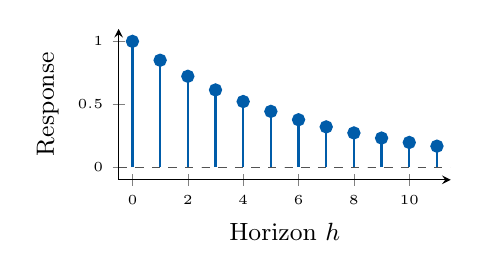
\begin{tikzpicture}
        \begin{axis}[
          width=5.8cm, height=3.5cm,
          xlabel={\small Horizon $h$},
          ylabel={\small Response},
          xmin=-0.5, xmax=11.5, ymin=-0.1, ymax=1.1,
          xtick={0,2,4,6,8,10},
          ytick={0,0.5,1},
          axis lines=left,
          tick label style={font=\tiny},
          label style={font=\small},
        ]
          \addplot[ycomb, color=unoblue, thick, mark=*, mark size=2pt,
                   samples at={0,1,...,11}] {0.85^x};
          \addplot[dashed, color=unogray, domain=-0.5:11.5] {0};
        \end{axis}
      \end{tikzpicture}\\[-3pt]
      \muted{\footnotesize\itshape Effect decays geometrically ($\rho^h$,
      here $\rho=0.85$); fades after $\approx 6$ periods.}
  \end{columns}
\end{frame}

% --- Slide: Forecasting with VAR ----------------------------------------------
\begin{frame}{Forecasting with VAR}
  \textbf{1-step ahead:}
  \[
    \hat{\mathbf{y}}_{T+1|T}
    = \hat{\mathbf{c}} + \hat{\mathbf{A}}_1\mathbf{y}_T
      + \cdots + \hat{\mathbf{A}}_p\mathbf{y}_{T-p+1}
  \]
  \textbf{Multi-step (recursive substitution):}
  \[
    \hat{\mathbf{y}}_{T+h|T}
    = \hat{\mathbf{c}} + \hat{\mathbf{A}}_1\hat{\mathbf{y}}_{T+h-1|T}
      + \cdots + \hat{\mathbf{A}}_p\hat{\mathbf{y}}_{T+h-p|T}
  \]
  using $\hat{\mathbf{y}}_{T+k|T} = \mathbf{y}_{T+k}$ for $k \leq 0$.
  \begin{keybox}
    VAR forecasts are particularly useful at short horizons and when
    cross-variable dynamics are strong. At long horizons the VAR
    reverts toward its unconditional mean, matching the theoretical
    property of stationary systems.
  \end{keybox}
  \muted{\footnotesize\itshape
    Socratic: if $a_{12} = a_{21} = 0$ in a VAR(1), what model does
    each equation reduce to?}
\end{frame}

% =============================================================================
\section{ARIMAX Models}
% =============================================================================

\sectionslide{ARIMAX Models}{%
  When the causal direction is clear, augment ARIMA with an
  exogenous predictor.}

% --- Slide: Regression with ARIMA errors --------------------------------------
\begin{frame}{Regression with ARIMA Errors}
  Standard OLS forecasting (Lecture 2) assumed independent errors.
  In practice, residuals are often autocorrelated.
  \begin{definitionbox}{ARIMAX / Regression with ARIMA Errors}
    {\small
    \[
      y_t = \underbrace{\mathbf{x}_t'\boldsymbol{\beta}}_{\text{regression}}
            + \underbrace{\eta_t}_{\text{ARIMA error}},
      \qquad \eta_t \sim \mathrm{ARIMA}(p,d,q)
    \]
    The error $\eta_t$ captures the autocorrelation \emph{not} explained
    by the regressors $\mathbf{x}_t$.}
  \end{definitionbox}
  \textbf{Why not use OLS?}
  \begin{itemize}\small
    \item OLS is unbiased but \emph{inefficient} (ignores error covariance)
    \item Standard errors are wrong $\Rightarrow$ invalid $t$-tests
          and prediction intervals (PIs)
    \item ARIMAX/SARIMAX jointly estimates $\boldsymbol{\beta}$ and
          the ARIMA parameters $(\phi,\theta)$ by MLE
          $\Rightarrow$ correct inference
  \end{itemize}
\end{frame}

% --- Slide: Dynamic regression ------------------------------------------------
\begin{frame}{Distributed Lag Effects}
  A \textbf{contemporaneous} regressor captures only the same-period effect:
  \[
    y_t = \beta_0 + \beta_1 x_t + \eta_t
  \]
  A \textbf{distributed lag} (DL) model captures delayed effects:
  \[
    y_t = \beta_0 + \beta_1 x_t + \beta_2 x_{t-1} + \cdots
          + \beta_{L+1} x_{t-L} + \eta_t
  \]
  \begin{columns}[T]
    \column{0.56\textwidth}
      \textbf{Example:} advertising spend $x_t$ affects sales $y_t$
      with a lagged carryover effect:
      \begin{itemize}\small
        \item $\beta_1$: immediate effect (same month)
        \item $\beta_2$: carryover from last month's ads
        \item Diminishing returns: $|\beta_1| > |\beta_2| > |\beta_3|$
      \end{itemize}
    \column{0.40\textwidth}
      \begin{keybox}
        {\small \textbf{Cross-correlation function (CCF):}
        $r_k = \mathrm{Corr}(x_t,\, y_{t+k})$.
        Bars outside ${\pm}1.96/\!\sqrt{T}$ indicate significant lag $k$.
        Select $L$ at the largest significant $k$; refine by AIC/BIC.}
      \end{keybox}
  \end{columns}
\end{frame}

% --- Slide: ARIMAX in Python --------------------------------------------------
\begin{frame}{ARIMAX: Practical Implementation}
  \textbf{Differencing rule:} if both $y_t \sim I(1)$ and $x_t \sim I(1)$,
  difference \emph{both} before fitting (unless cointegrated --- see below).
  \begin{keybox}
    \textbf{Python:} \texttt{statsmodels.tsa.statespace.sarimax.SARIMAX}
    accepts an \texttt{exog} argument for exogenous regressors.\\[3pt]
    \texttt{SARIMAX(y, exog=X, order=(p,d,q),}
    \texttt{seasonal\_order=(P,D,Q,m)).fit()}
  \end{keybox}
  \textbf{Model selection workflow:}
  \begin{enumerate}\small
    \item Unit-root test $y_t$ and $x_t$ separately $\to$ choose $d$
    \item Plot CCF of $(\Delta^d y_t)$ vs.\ $(\Delta^d x_t)$ $\to$
          choose lag $L$
    \item Identify ARIMA$(p,d,q)$ for residuals via ACF/PACF
    \item Select $(p,q)$ by AIC; check residuals with Ljung-Box
  \end{enumerate}
  \muted{\footnotesize\itshape
    Socratic: if $x_t$ is I(1) but $y_t$ is I(0), should you
    difference $x_t$ before including it as a regressor?}
\end{frame}

% --- Slide: VAR vs ARIMAX -----------------------------------------------------
\begin{frame}{VAR vs.\ ARIMAX: When to Use Which}
  \begin{center}
    {\small
    \begin{tabular}{lll}
      \toprule
      \textbf{Feature} & \textbf{VAR} & \textbf{ARIMAX} \\
      \midrule
      Direction of causality & Unknown / symmetric & Known (unidirectional) \\
      Number of variables    & Any $k$ (keep $k\leq 4$) & 1 outcome + regressors \\
      Feedback loops         & Allowed                   & Not modeled \\
      Interpretability       & IRF, FEVD$^\dagger$       & Regression coefficients \\
      Forecasting $x_t$      & Joint (endogenous)        & Needs external forecast \\
      \midrule
      Preferred when\ldots   & Macro / finance; symmetric & Clear cause $\to$ effect \\
      \bottomrule
    \end{tabular}
    }
  \end{center}
  \muted{\footnotesize\itshape $^\dagger$FEVD = forecast error variance
  decomposition: fraction of $y_j$'s forecast variance explained by shocks
  to $y_i$ at each horizon.}
  \begin{warningbox}
    ARIMAX treats $x_t$ as \textbf{exogenous}: it assumes $x_t$ does not
    respond to past $y_t$. If feedback exists, use VAR instead --- otherwise
    forecasts of $y_t$ will require an external forecast of $x_t$.
  \end{warningbox}
\end{frame}

% =============================================================================
\section{Cointegration and Error Correction}
% =============================================================================

\sectionslide{Cointegration and Error Correction}{%
  Two non-stationary series that share a long-run trend can be modeled
  together without differencing away their relationship.}

% --- Slide: Spurious regression revisited ------------------------------------
\begin{frame}{Spurious Regression Revisited}
  \textbf{Recall from Lecture 2,} \textcite{GrangerNewbold1974}: regressing
  independent random walks yields spuriously high $R^2$.
  But some I(1) pairs are \emph{genuinely} linked.
  \begin{columns}[T]
    \column{0.52\textwidth}
      {\small\textbf{Spurious:} independent RWs diverge over time}\\[2pt]
      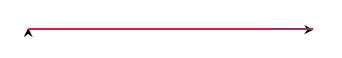
\begin{tikzpicture}
        \begin{axis}[
          width=5.2cm, height=1.6cm,
          xmin=0, xmax=10, ymin=-4.5, ymax=5.5,
          axis lines=left, xtick=\empty, ytick=\empty,
          tick style={draw=none},
        ]
          \addplot[color=unoblue, thick, line width=0.9pt] coordinates {
            (0,0)(1,0.5)(2,1.2)(3,1.8)(4,2.1)(5,2.8)
            (6,3.2)(7,3.8)(8,4.5)(9,4.2)(10,5.0)};
          \addplot[color=unored, thick, line width=0.9pt] coordinates {
            (0,0)(1,-0.3)(2,-0.8)(3,-1.5)(4,-2.0)(5,-1.8)
            (6,-2.5)(7,-3.0)(8,-2.8)(9,-3.5)(10,-4.0)};
        \end{axis}
      \end{tikzpicture}
      \\[3pt]
      {\small\textbf{Cointegrated:} common trend,
      $y_t - \beta x_t \sim I(0)$}\\[2pt]
      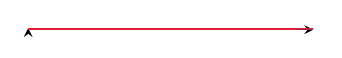
\begin{tikzpicture}
        \begin{axis}[
          width=5.2cm, height=1.6cm,
          xmin=0, xmax=10, ymin=-0.5, ymax=4.8,
          axis lines=left, xtick=\empty, ytick=\empty,
          tick style={draw=none},
        ]
          \addplot[color=unoblue, thick, line width=0.9pt] coordinates {
            (0,0)(1,0.5)(2,1.0)(3,1.5)(4,1.8)(5,2.2)
            (6,2.5)(7,3.0)(8,3.2)(9,3.8)(10,4.0)};
          \addplot[color=unored, thick, line width=0.9pt] coordinates {
            (0,0.2)(1,0.8)(2,1.1)(3,1.7)(4,1.6)(5,2.4)
            (6,2.3)(7,3.1)(8,3.0)(9,3.5)(10,4.2)};
        \end{axis}
      \end{tikzpicture}
    \column{0.44\textwidth}
      \begin{keybox}
        {\small \textbf{Engle--Granger test}
        \parencite[][Ch.~19]{Hamilton1994}:\\[3pt]
        1.\ Regress $y_t$ on $x_t$ (levels)\\
        2.\ Residuals $\hat{e}_t = y_t - \hat{\beta}x_t$\\
        3.\ Augmented Dickey-Fuller (ADF) on $\hat{e}_t$:\\
        \phantom{3.\ }Reject unit root $\Rightarrow$ cointegrated
        }
      \end{keybox}
      \muted{\footnotesize\itshape
        Example: income \& consumption --- both I(1),
        but $c_t - \beta y^d_t \sim I(0)$
        (consumption tracks income in the long run).}
  \end{columns}
\end{frame}

% --- Slide: Error Correction Model -------------------------------------------
\begin{frame}{The Error Correction Model (ECM)}
  If $y_t$ and $x_t$ are cointegrated with equilibrium
  $y_t = \beta x_t + u_t$ ($u_t \sim I(0)$):
  \begin{definitionbox}{Error Correction Model}
    {\small
    \[
      \Delta y_t
      = \underbrace{\alpha(y_{t-1} - \beta x_{t-1})}_{\text{error correction}}
      + \underbrace{\gamma_1 \Delta y_{t-1} + \delta_1 \Delta x_{t-1}
                   + \cdots}_{\text{short-run dynamics}}
      + \varepsilon_t
    \]
    $\alpha < 0$: speed of adjustment;
    $\gamma_1$: own short-run lag; $\delta_1$: cross short-run lag.
    If $y_{t-1}$ is \emph{above} equilibrium, the ECM term pushes
    $\Delta y_t < 0$ (mean-reverting).}
  \end{definitionbox}
  \begin{columns}[T]
    \column{0.56\textwidth}
      \begin{itemize}\small
        \item ECM captures \emph{both} short-run dynamics and
              long-run equilibrium in one model
        \item Differenced variables $\Rightarrow$ no spurious regression
        \item Error correction term $\Rightarrow$ no loss of long-run info
      \end{itemize}
    \column{0.40\textwidth}
      \begin{warningbox}
        {\small \textbf{Do not} difference cointegrated series before
        regression --- this discards the long-run relationship.}
      \end{warningbox}
  \end{columns}
  \muted{\footnotesize\itshape
    Example: $\hat{\alpha}=-0.3$, $y_{t-1}-\hat{\beta}x_{t-1}=+2.0$
    (10\% above equilibrium) $\Rightarrow$ ECM contributes
    $-0.3\times 2.0 = -0.6$ to $\Delta y_t$ (partial correction).}
\end{frame}

% =============================================================================
\section{Key Takeaways and Roadmap}
% =============================================================================

% --- Slide: Key Takeaways -----------------------------------------------------
\begin{frame}{Key Takeaways}
  \begin{keybox}
    {\small
    \begin{enumerate}
      \item \textbf{Granger causality:} $x_t$ Granger-causes $y_t$ if
            $x_t$'s past improves forecasts of $y_t$ beyond $y_t$'s own past.
      \item \textbf{VAR:} symmetric multivariate model estimated
            equation-by-equation; use IRF to trace shock propagation;
            keep $k$ small.
      \item \textbf{ARIMAX:} augment ARIMA with exogenous regressors when
            causal direction is clear; use SARIMAX in statsmodels.
      \item \textbf{Cointegration:} two I(1) series with a stable long-run
            relationship --- model as ECM, not as levels or differences alone.
      \item \textbf{Model choice:} symmetric dynamics $\to$ VAR; clear cause
            $\to$ ARIMAX; long-run equilibrium $\to$ ECM.
    \end{enumerate}
    }
  \end{keybox}
  \muted{\footnotesize\itshape
    VAR(1) with $a_{12}=a_{21}=0$ collapses to two independent AR(1) models
    --- the multivariate framework nests the univariate special case.}
\end{frame}

% --- Slide: What's Next -------------------------------------------------------
\begin{frame}{What's Next: Forecast Evaluation}
  We now have five model families:
  \begin{itemize}\small
    \item Benchmarks (na\"{i}ve, seasonal na\"{i}ve, mean, drift)
    \item Regression and AR models (Lecture 2)
    \item Exponential smoothing / ETS (Lecture 3)
    \item ARIMA / SARIMA (Lecture 4)
    \item VAR, ARIMAX, ECM (Lecture 5)
  \end{itemize}
  \vspace{0.1cm}
  \textbf{Key question:} how do we rigorously compare these models
  out-of-sample?
  \begin{keybox}
    \textbf{Lecture 6:} Forecast evaluation --- walk-forward validation,
    the Diebold-Mariano test \parencite{Diebold1995}, and forecast
    combination.
  \end{keybox}
  \begin{center}
    \muted{\small
    \textbf{Lab 5:} Granger causality tests, VAR fitting and IRF,
    ARIMAX on RSXFS + consumer sentiment.
    }
  \end{center}
\end{frame}

% --- References ---------------------------------------------------------------
\begin{frame}[allowframebreaks]{References}
  \printbibliography[heading=none]
\end{frame}

\end{document}
